\documentclass[a4paper,12pt, oneside, twocolumn]{scrartcl}
%\usepackage[ngerman]{babel}
\usepackage[utf8]{inputenc}
\setlength{\parindent}{0em}
\usepackage{eurosym}
\usepackage{amsmath}
\usepackage{amssymb}
\usepackage{dsfont}
\usepackage{polynom}
\usepackage{graphicx}
\usepackage{caption}
\usepackage{tikz}
\usepackage[a4paper,portrait,left=1.0cm,right=1.0cm,top=2cm,bottom=2cm]{geometry}
\usepackage{pgf} % Zur Einbindung der PGF Files
\usepackage{bm}

\usepackage{algorithm}
\usepackage{algpseudocode}

\newcommand{\e}[1]{\text{e}^{#1}}
\newcommand{\rot}[2][rot]{\textcolor{#1}{#2}}
\newcommand{\gruen}[2][gruen]{\textcolor{#1}{#2}}
\newcommand{\frontcolor}[2][frontcolor]{\textcolor{#1}{#2}}
\newcommand{\gelb}[2][gelb]{\textcolor{#1}{#2}}
\newcommand{\orange}[2][orange]{\textcolor{#1}{#2}}
\newcommand{\blau}[2][blau]{\textcolor{#1}{#2}}
\newcommand{\hellblau}[2][hellblau]{\textcolor{#1}{#2}}
\newcommand{\lila}[2][lila]{\textcolor{#1}{#2}}
\newcommand{\dunkelrot}[2][dunkelrot]{\textcolor{#1}{#2}}
\newcommand{\dunkelgelb}[2][dunkelgelb]{\textcolor{#1}{#2}}

%%%%%%%%%%%%%%%%%%%%%%%%%%%%%%%%%%%%%%%%%%%%%%%%%%%%%%%%%%%%%%%%%%%%%%%
\newcommand{\norm}[1]{\left\lVert#1\right\lVert}
\newcommand{\dv}{\thinspace \mathrm{d}v}
\newcommand{\dw}{\thinspace \mathrm{d}w}
\newcommand{\dx}{\thinspace \mathrm{d}x}
\newcommand{\dy}{\thinspace \mathrm{d}y}
\newcommand{\dt}{\thinspace \mathrm{d}t}
\newcommand{\dr}{\thinspace \mathrm{d}r}
\newcommand{\ds}{\thinspace \mathrm{d}s}
\newcommand{\du}{\thinspace \mathrm{d}u}
\newcommand{\dz}{\thinspace \mathrm{d}z}
\newcommand{\dW}{\thinspace \mathrm{d}W}
\newcommand{\dX}{\thinspace \mathrm{d}X}
\newcommand{\dP}{\thinspace \mathrm{d}P}
\DeclareMathOperator*{\esssup}{ess\,sup}
\DeclareMathOperator*{\argmin}{arg\,min}

% Light Mode Customization
\usepackage{xcolor}
%\definecolor{backgroundgray}{RGB}{255,255,255}  % Weiß als Seitenhintergrund
\definecolor{textwhite}{RGB}{0,0,0}            % Schwarz als globale Schriftfarbe
\definecolor{boxgray}{RGB}{245,245,245}        % Sehr helles Grau für Box-Hintergründe
\definecolor{boxframe}{RGB}{200,200,200}       % Helles Grau für Box-Rahmen
\pagecolor{boxgray}  % Hintergrund auf Weiß
\color{textwhite}           % Text auf Schwarz

% Eigene Farben definiert (nun optimiert für hellen Hintergrund)
\definecolor{rot}{RGB}{204,0,0}
\definecolor{blau}{RGB}{0,102,204}
\definecolor{orange}{RGB}{204,85,0}
\definecolor{gruen}{RGB}{0,153,0}
\definecolor{dunkelgruen}{RGB}{0,153,0}
\definecolor{dunkelblau}{RGB}{0,128,128}
\definecolor{backcolor}{RGB}{235,245,255}
\definecolor{frontcolor}{RGB}{0,153,0}
\definecolor{hellblau}{RGB}{180,210,235}
\definecolor{lila}{RGB}{153,0,153}
\definecolor{gelb}{RGB}{204,153,0}
\definecolor{dunkelrot}{RGB}{153,0,51}
\definecolor{dunkelgelb}{RGB}{153,153,0}
\usepackage[backend=biber,style=numeric]{biblatex}
\addbibresource{references.bib}

% Ränder und Layout für geteilte Ansicht
\usepackage{multicol}
\setlength{\columnsep}{1cm}  % Abstand zwischen den Spalten

% Keine Seitenzahl
\pagestyle{empty}

% Begin des Dokuments
\begin{document}

\vspace{-1em} % Reduzierter Abstand

\section*{Actor-Critic Methods for Control Problems}

% Schemata Actor-Critic Methode
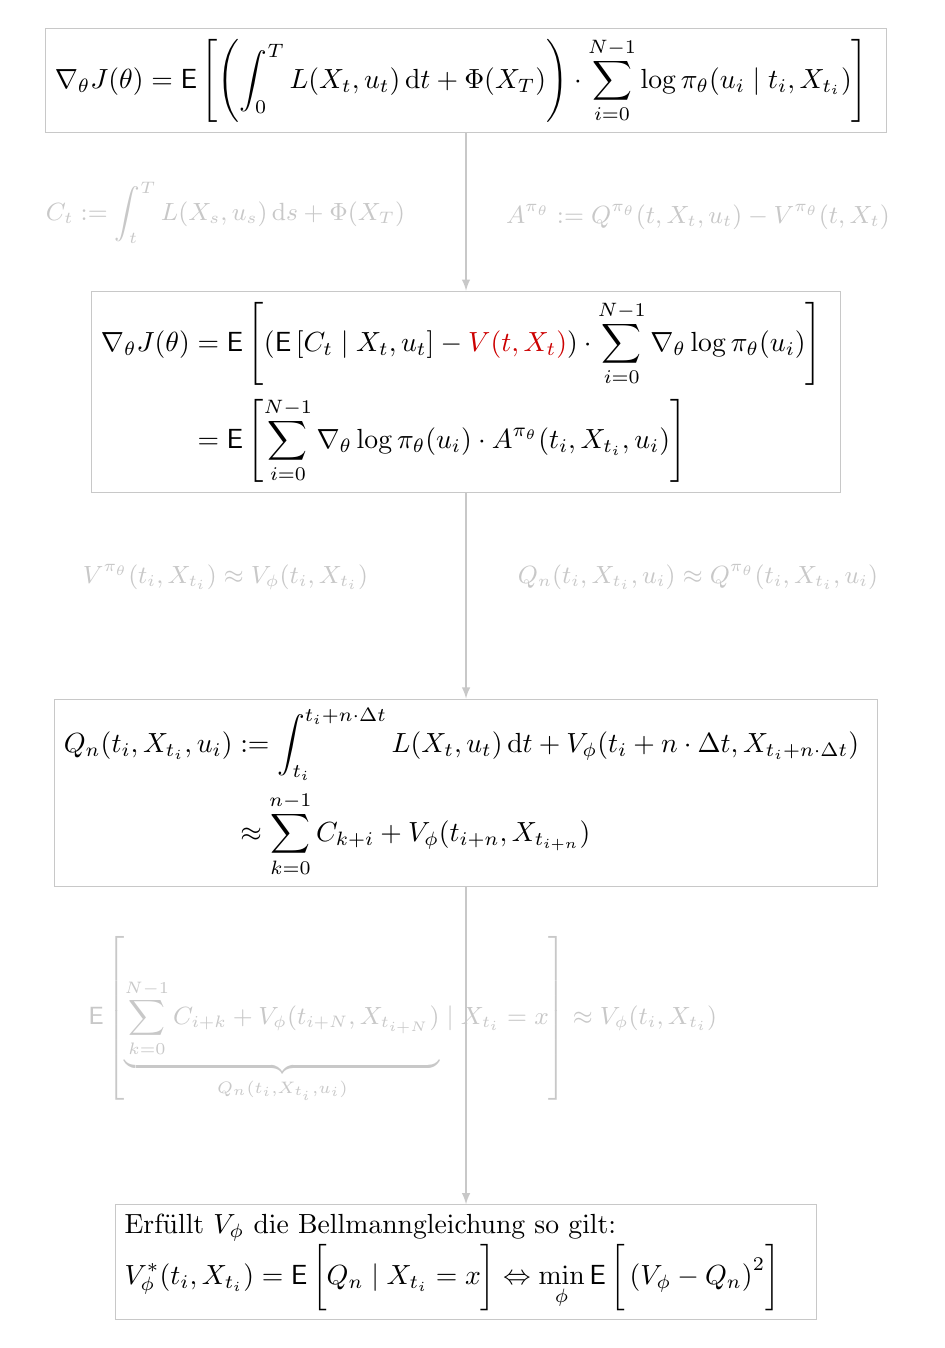
\begin{tikzpicture}[>=latex]
    \node[draw= boxframe,anchor = north ,align=left] (a) at (0,0) {
        %
        $\begin{aligned}
            \nabla_{\theta} J(\theta)
            =
            \mathsf{E}
            \left[
                \left(
                    \int_{0}^{T} L(X_t,u_t) \dt + \Phi(X_T)
                \right)
                \cdot
                \sum_{i=0}^{N-1} \log \pi_{\theta}(u_i \mid t_i, X_{t_i}) 
            \right]
        \end{aligned}$
    };
    \node[draw = boxframe, anchor=north, align=left] (b) at 
    ([yshift=-2.0cm, xshift=-0.0cm]a.south) {
        $\begin{aligned}
            \nabla_{\theta} J(\theta)
            &= 
            \mathsf{E}
            \left[
                \left(
                \mathsf{E}
                \left[
                    C_t \mid X_t, u_t
                \right]
                - \rot{V(t,X_t)}
                \right)
                \cdot
                \sum_{i=0}^{N-1}
                \nabla_{\theta} \log \pi_\theta (u_i) 
            \right]
            \\
            &=
            \mathsf{E}
            \left[
                \sum_{i=0}^{N-1}
                \nabla_{\theta} \log \pi_\theta (u_i) 
                \cdot
                A^{\pi_{\theta}}(t_i,X_{t_i},u_i)
            \right]
        \end{aligned}$
    };
    \node[draw= white,anchor = north ,align=left] (a1) at 
    ([yshift=-0.5cm, xshift=-3.0cm]a.south) {
    %
        \small{
            $\begin{aligned}
                \color{boxframe}{C_t := \int_{t}^{T} L(X_s,u_s) \ds + \Phi(X_T)}
            \end{aligned}$
        }
    };
    \node[draw= white,anchor = north ,align=left] (a2) at 
    ([yshift=-0.75cm, xshift=3.0cm]a.south) {
    %
        \small{
            $\begin{aligned}
                \color{boxframe}{A^{\pi_{\theta}}:= Q^{\pi_{\theta}}(t,X_t,u_t) - V^{\pi_{\theta}}(t,X_t)}
            \end{aligned}$
        }
    };
    \node[draw = boxframe, anchor=south, align=left] (c) at 
    ([yshift=-5.0cm, xshift=-0.0cm]b.south) {
        $\begin{aligned}
            Q_n(t_i , X_{t_i}, u_i) 
            &:= 
            \int_{t_i}^{t_i + n \cdot \Delta t} L(X_t,u_t) \dt 
            + 
            V_{\phi}(t_i + n \cdot \Delta t, X_{t_i + n \cdot \Delta t})
            \\
            &\approx
            \sum_{k=0}^{n-1}
            C_{k+i}
            +
            V_{\phi}(t_{i+n}, X_{t_{i+n}})
        \end{aligned}$
    };
    \node[draw= white,anchor = north ,align=left] (b1) at 
    ([yshift=-0.75cm, xshift=-3.0cm]b.south) {
    %
        \small{
            $\begin{aligned}
                \color{boxframe}{V^{\pi_{\theta}}(t_i,X_{t_i}) \approx V_{\phi}(t_i,X_{t_i})}
            \end{aligned}$
        }
    };
    \node[draw= white,anchor = north ,align=left] (b2) at 
    ([yshift=-0.75cm, xshift=3.0cm]b.south) {
    %
        \small{
            $\begin{aligned}
                \color{boxframe}{Q_n(t_i,X_{t_i},u_i) \approx Q^{\pi_{\theta}}(t_i,X_{t_i},u_i)}
            \end{aligned}$
        }
    };
    \node[draw= white,anchor = north ,align=left] (c1) at 
    ([yshift=-0.5cm, xshift=-0.75cm]c.south) {
    %
        \small{
            $\begin{aligned}
                \color{boxframe}{
                    \mathsf{E}
                    \left[
                        \underbrace{
                            \sum_{k=0}^{N-1} C_{i+k}
                            + 
                            V_{\phi}(t_{i+N}, X_{t_{i+N}})
                        }_{
                            Q_n(t_i , X_{t_i}, u_i)
                        }
                        \mid
                        X_{t_i}= x
                    \right] \approx V_{\phi}(t_i , X_{t_i})
                    }
            \end{aligned}$
        }
    };
    \node[draw = boxframe, anchor=south, align=left] (d) at 
    ([yshift=-5.5cm, xshift=-0.0cm]c.south) {
        Erfüllt $V_{\phi}$ die Bellmanngleichung so gilt: \\
        $\begin{aligned}
            V_{\phi}^{*} (t_i , X_{t_i}) 
            &=
            \mathsf{E}
            \left[
                \vphantom{\int}
                Q_n
                \mid
                X_{t_i}= x
            \right]
            \Leftrightarrow
            \min_{\phi}
            \mathsf{E}
            \left[
                \vphantom{\int}
                \left(
                    V_{\phi}
                    -
                    Q_n
                \right)^2
            \right]
        \end{aligned}$
    };
    \draw[->, color = boxframe] (a) -- (b);
    \draw[->, color = boxframe] (b) -- (c);
    \draw[->, color = boxframe] (c) -- (d);
    %\draw[->, color = gruen] (a.south) -- ++(0cm, -4.7cm);
\end{tikzpicture}


\section*{Solving a (Stochastic) Control Problem}

\begin{align*}
    \min_{\pi} \mathsf{E}
    \left[
        \int_0^1 X_t +u_t^2  \dt + X_1^2  
    \right]
    \quad 
    \dX_t = (X_t + u_t + 1) \dt + \sigma \dW_t, 
    \quad 
    u_t \sim \pi_{\theta}(\cdot \mid t)
\end{align*}

\section*{Further Directions}

Further improvements based on \cite{lillicrap2015ddpg},
\cite{haarnoja2018sac} and \cite{haarnoja2018sacapps}.

\small
\printbibliography

\end{document}